\begin{savequote}[75mm]
Nulla facilisi. In vel sem. Morbi id urna in diam dignissim feugiat. Proin molestie tortor eu velit. Aliquam erat volutpat. Nullam ultrices, diam tempus vulputate egestas, eros pede varius leo.
\qauthor{Quoteauthor Lastname}
\end{savequote}

\chapter{Basic characterizations}
% fig:2p_retino
% fig:rf_examples
% fig:retino_scatter
% fig:rf_aggregate
% fig:vf_coverage

% fig:gratings_examples
% fig:gratings_aggregate
% fig:theta_vs_rf_angle

% Supps:
% rf5_v_rf10
% spherical_correction
% gratings_fitting
% vf_targeting

\newthought{Beyond V1}, a subset of contiguous areas spanning the lateral edge of rat cortex have garnered significant attention over the past few years due to similarities between these areas in the rat and the primate ventral visual stream. Several studies \cite{Vermaercke2014, Tafazoli2017, Vinken2016NeuralCortex} have investigated these visual areas specifically in the context of visual object representations in order to test the extent to which single-unit properties characteristic of the highest levels of the primate ventral stream might also be found in the rat. These previous studies bolster the promise of the rat visual system as highly sophisticated, perhaps similar to that of primates in certain ways. 
However, monkeys and rodents differ in dramatic ways --- on one hand, similarities in how their visual systems solve a given problem are incredibly exciting, as they point to general principles conserved across specie. On the other hand, each solution is likely to be influenced by differences in the natural visual statistics by which their visual systems have been shaped. 

Despite the fact that animals with the best vision, like cats or monkeys, have been the traditional models of choice for vision studies, mice have become increasingly popular models for studying visual circuits over the past decade. This is arguably due to the immensely powerful genetic tools combined with chronic, large-scale population recordings, much of which are prohibitively challenging to use in monkeys.

In contrast, although rats have long been studied for visually-guided behaviors, large-scale cellular resolution access to their visual cortex has proved to be far more challenging. Our broad-level goal is to bridge the gap between neural circuit access and rich behavioral capacities in the rat. What has remained lacking is a basic characterization of any visual area beyond V1 in the rat. Such a systematic study provides valuable points of comparison not just with primates, but with other animal models, including mice. 

% Broad overview of experiment design
Two overarching goals shaped our experimental design (Figure\ref{fig:experiment_design}). First, we hoped to contribute an immensely powerful method to the existing body of literature on visual object recognition in rats. Several studies have characterized single-unit response properties of lateral extrastriate areas in rats that may be similar to those found in the primate ventral stream\cite{Tafazoli2017, Vermaercke2014, VinkenX, Vermaerke2015}. As such, we know relatively more about single-unit response properties in these lateral areas than in any other extrastriate area of the rat\cite{Vermaercke2014, Tafazoli2017, Vinken2016, REFREF}. To be able to compare our findings with previous electrophysiology studies, we focused on areas V1, LM, and LI. 

At the same time, much less is known about more basic response properties of these visual areas. As a parallel goal, we sought to provide a first comprehensive survey of basic, visual response properties across these different cortical areas in the rat using optical imaging. 

% Figure:  Experimental design.
\begin{figure}
    \includegraphics[width=\textwidth]{figures/chapter_3/experiment_design/experiment_design.pdf}
    \vspace{.1in}
    \caption[Experiment design]{Experiment design for characterizing visual responses in rat lateral cortex. \textbf{A.} 
    \label{fig:experiment_design}}
\end{figure}

Using a large battery of visual stimuli, we characterized basic visual response properties of these areas for the first time with cellular resolution imaging. In the same sessions, we also tested a subset of the complex visual object stimuli used to test the perceptual behavior of rats (described in Chapter 1). At a broader level, that they may be capable of supporting visual object recognition behavior is an exciting starting point for combining the powerful tools common in traditional genetic models like mice with kinds of complex behaviors associated with primates.  

\section{Identification of two-photon imaging sites}
The mirror reflections of the retinotopic gradient in our wide-field maps identified macro-level areal borders. We used these maps to determine which visual areas to target for two-photon imaging sessions. In order to register the two-photon maps to the wide-field maps, we acquired an anatomical volume at the start of each session. This was a surface-level z-stack that captured fiduciary markers in both channels: while the green channel was always used for functional runs (GCaMP), we used the red channel to acquire images of blood vessels filled with a temporary fluorescent dye that was injected at the start of each session (see Methods). If blood vessel images were unavailable, the green channel could be used for registration. 

Each rat underwent localizer and functional runs (Figure\ref{fig:experiment_design}). Localizer runs were conducted on a day prior to full functional sessions. These sessions were used to identify which parts of the visual field corresponded to a given imaging site, targeted based on the surface-level vasculature and wide-field areal mapping (see Chapter 2 REFREF). Two-photon vasculature images were matched offline to the high-resolution images we took of the brain surface in each wide-field mapping session (Figure\ref{fig:2p_retino}). We selected matching points between the two views based on uniquely identifiable blood vessels present in both images, then used these points to identify a transformation matrix to warp one into the other (see Methods).

We used two types of mapping protocols that targeted different scales of retinotopic organization. The first captured broad retinotopic preferences across the field-of-view using the same sweeping bar stimulus used to identify area borders in wide-field maps. The second provided a more fine-scaled characterization of individual receptive fields for each neuron in the selected FOV. In addition, since only a subset of the experiments used full-field stimuli, it was important to accurately identify the region of visual space to which most cells in a given FOV were responsive and target the stimulus presentation there. 

Once a given FOV was identified as visually responsive, and the receptive field locations of the whole population could be identified, functional runs were conducted in subsequent days. We selected a battery of stimuli to provide a foundation for basic visual response properties in the lateral extrastriate areas of the rat. The final stimulus sets included drifting gratings of multiple orientations, spatial frequencies, and speeds, and a subset of the complex object stimuli used to test rats' perceptual behavior (as described in Chapter 1, REFREF). In addition, both of the localizer stimuli were re-tested in the same session as these functional runs.

% ---------------------------------------------------------------
% 2p retinotopy
% ---------------------------------------------------------------
\section{Fine-scale retinotopic organization in rat lateral cortex}
The particular region and extent of visual space that a patch of cortex represents has important implications for its function. For example, in primates, most areas of the ventral stream over-represent the central visual field, enhancing the processing of features near the fovea\cite{REFREF, Gattass2005CorticalDynamics}. Although mice and rats do not have foveal vision, several groups have shown biases of visual field coverage across visual cortex in mice\cite{Garrett2014, Marshel2011, REFREF}. 

% 2p retinotopy -------------------------------------------------
% fig:2p_retino (2p setup, coregistration, gradient, cortical mag)
\subsection{Cortical magnification}

Using the same phase-encoding Fourier paradigm we used to measure retinotopic gradients in wide-field maps, we characterized retinotopic preferences across a given two-photon field-of-view (FOV). This method also allowed us to quickly identify and validate that the expected retinotopic gradient direction was present across the two-photon FOV (see Figure\ref{fig:2p_retino}).

% fig:2p_retino (Schematic, coregistration, retinotopy)
\begin{figure}
    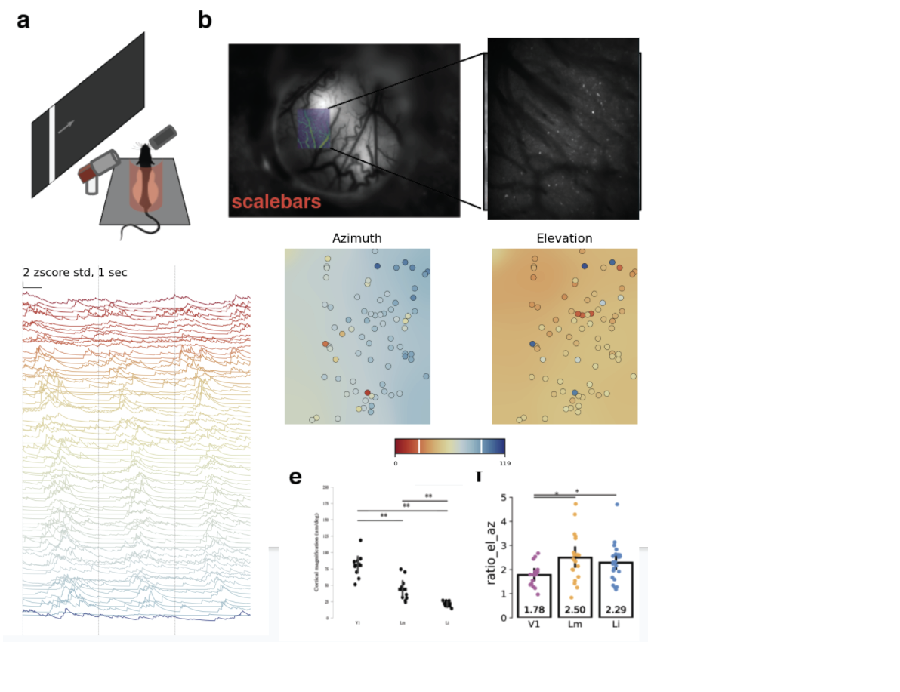
\includegraphics[width=\textwidth]{figures/chapter_3/2p_retino/2p_retino.pdf}
    \vspace{.1in}
    \caption[Identification of areas with two-photon imaging]{Coregistration and area identification for two-photon imaging. \textbf{A.} Schematic of imaging experiments in awake, head-fixed rats. \textbf{B.} \textit{Left}: Wide-field image of the surface vasculature in the cranial window of an example rat. The overlay shows the co-registered anatomical image of the surface vasculature acquired by two-photon imaging. \textbf{C.} Example two-photon imaging field-of-view using the standard, large-FOV mode (scale bar, $100um$ REFREF). 
    \label{fig:2p_retino}}
\end{figure}

% Cortical magnification
We observed retinotopic gradients across visual axes of elevation (ventral-dorsal) and azimuth (nasal-temporal) for large two-photon FOVs ($~1mm^2$) imaged in areas V1, LM, and LI (Figure\ref{fig:2p_retino}). To quantify how much cortex is devoted to a given unit of visual space in rat extrastriate areas, we measured cortical magnification in areas V1, LM and LI. Overall, we found that cortical magnification decreased from V1 to LM to LI, consistent with the expectation that larger areas have more cortical real estate for representing a given part of visual space (Figure\ref{fig:2p_retino}\textbf{a}). 

Cortical magnification is not necessarily isotropic, \textit{i.e.}, similar magnification along vertical (azimuth) and horizontal (elevation) axes of the visual field. We found an asymmetric expansion along the vertical dimension of visual space in rat V1, as well as in areas LM and LI (Figure\ref{fig:2p_retino}\textbf{b}). The degree to which the cortical representation of the vertical dimension was expanded relative to that of the horizontal dimension was significantly greater for LM and LI than for V1 (LM: p<0.05, LI: p<0.01 REFREF). This asymmetry is consistent with findings in mouse V1, in which several studies have reported an expanded representation alon the vertical dimension of visual space\cite{Garrett2014, Liang2018, Bonin2011}.  

% ---------------------------------------------------------------
% Receptive fields + scatter
% ---------------------------------------------------------------
% fig:rf_examples
% fig:retino_scatter
% fig:rf_aggregate
% fig:vf_coverage

\subsection{Receptive fields are anisotropic}
% Retino scatter
While previous studies have relied on coarse retinotopy to identify the areas in which they were recording, the fine-scale retinotopic organization of cell bodies in any extrastriate area remains unknown. REFREF Previous studies in mouse visual areas indicate the presence of a fine-scale retinotopic scatter from retinal ganglion cell (RGC) inputs, through the lateral geniculate nucleus (LGN), and into V1 and LM\cite{Liang2018, Andermann2011, Marques2018}. However, it remains unknown whether this scatter is present in other extrastriate areas of rodent cortex, whether and to what extent rat visual areas also exhibit scatter, and whether this is functionally advantageous in any way or random biological noise.

% fig:rf_examples
\begin{figure}[t!]
    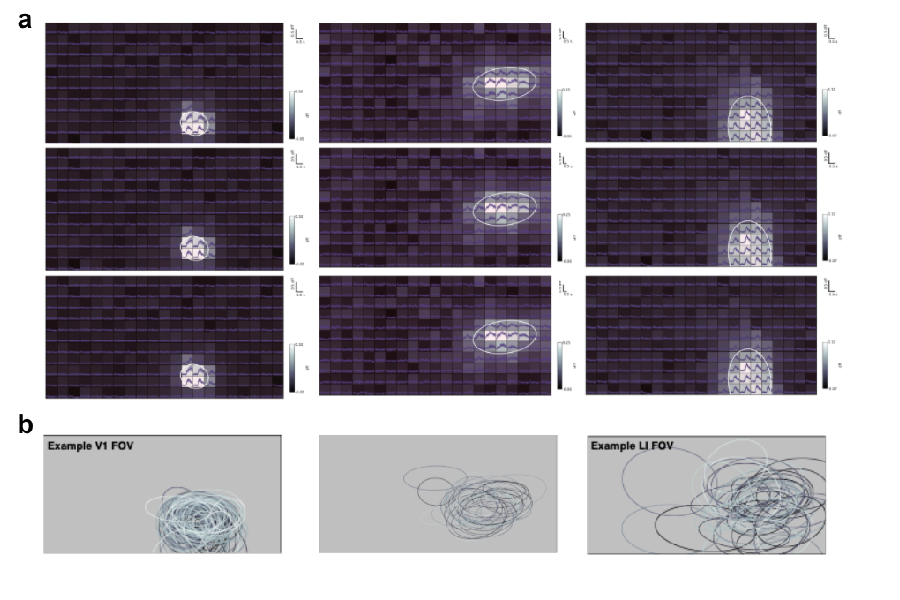
\includegraphics[width=\textwidth]{figures/chapter_3/rf_examples/rf_examples.pdf}
    \vspace{.1in}
    \caption[Receptive field mapping]{Mapping receptive fields of single neurons. \textbf{A.} REFREF.
    \label{fig:rf_examples}}
\end{figure}

In order to more finely characterize retinotopic preferences of individual cells, we quantified receptive field (RF) properties by stimulating tiled locations across the visual field (Figure\ref{fig:rf_examples}). We used tile sizes of 5 or 10 degrees of visual angle to account for the possibility that cells with larger receptive fields may not be effectively stimulated by small stimuli, and vice versa, that  cells with small receptive fields may have overestimated receptive field sizes if the tiling resolution is too large.

We mapped RFs in X\%, X\% and X\% of cells imaged in V1 (REFREF of REFREF neurons, REFREF imaging locations, REFREF rats), LM (REFREF), and LI (REFREF), respectively. Consistent with previous electrophysiology measures\cite{Vermaercke2014, Tafazoli2017}, overall receptive field sizes increased from V1 to LM to LI (REFREF).

% ---------------------------------------------------------------
% RF properties
% ---------------------------------------------------------------
% RFs are anisotropic, elongated along azimuth
Given the observed asymmetry in cortical magnification along azimuth and elevation (see Figure\ref{fig:retino_scatter}), we asked whether this asymmetry was also present at the level of individual cells. Interestingly, most receptive fields exhibited some degree of anisotropy, with receptive field angles biased toward 0 degrees, elongated along azimuth (Figure\ref{fig:rf_aggregate}). 
% However, we did not observe strong relationships between anisotropy and retinotopic scatter (REFREF, Supplemental 3.3) nor between angular bias in anisotropy (horizontally or vertically anisotropic, see Methods) and retinotopic position (REFREF, Supplemental 3.4). 
-Sit & Goard, bias for cells representing LOWER visual field, stronger coherent motion response -- spatial asymmetry in motion representation/sensitivity

\begin{figure}[t!]
    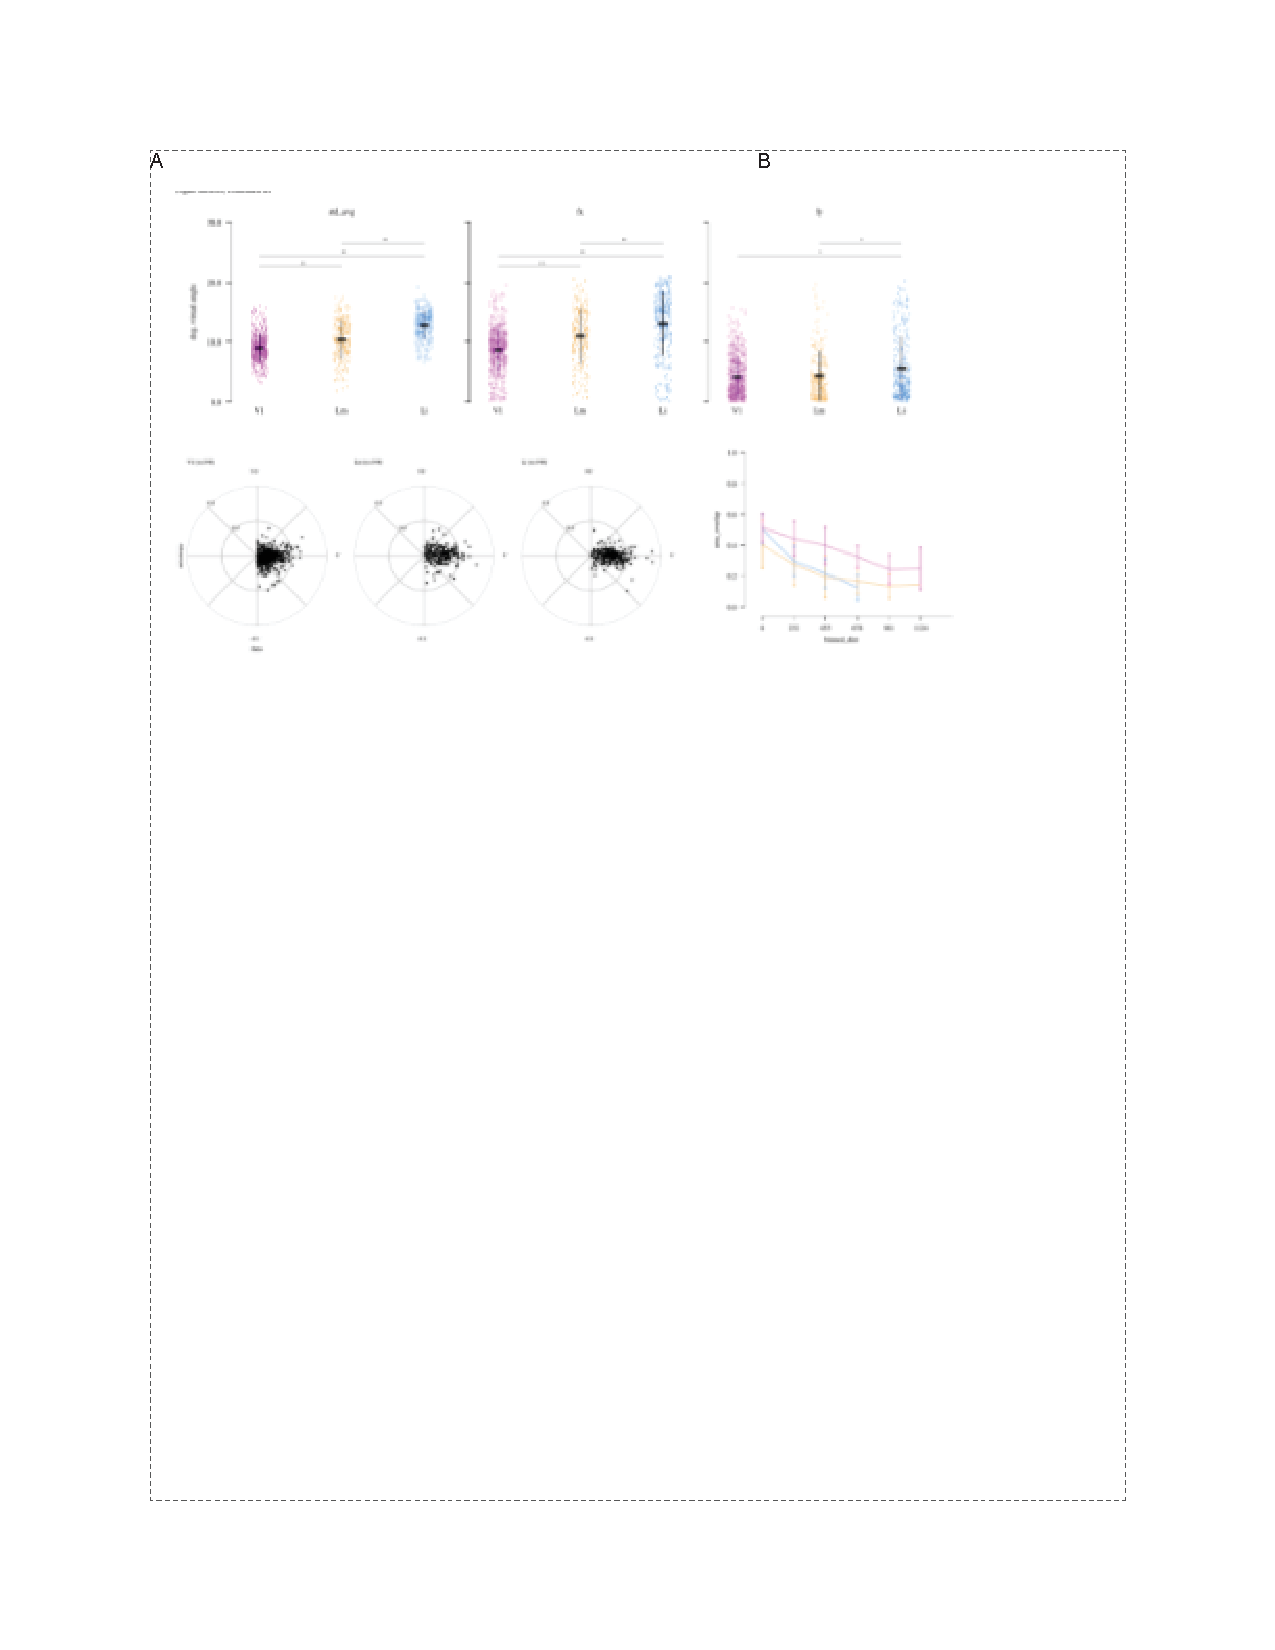
\includegraphics[width=\textwidth]{figures/chapter_3/rf_aggregate/rf_aggregate.pdf}
    \vspace{.1in}
    \caption[Receptive field properties]{Receptive field properties across lateral extrastriate cortex. \textbf{A.} REFREF.
    \label{fig:rf_examples}}
\end{figure}

% Spherical correction check
To confirm that the observed receptive field anistropy was not simply due to variable screen distance, we calculate the same metrics with a spherical correction. Typically, in visual field mapping studies, the screen is close enough to the animal's eye that significant warping can occur at the edges of the visual field, relative to the portions directly in front of the animal, producing a "fishbowl" effect. Experimenters often correct for this distortion by presenting an inversely distorted stimulus, effectively reversing the warped appearance (see Figure\ref{fig:spherical_correction}). 

Alternatively, the stimuli can be presented as is, on the flat monitor, and the measured responses can be transformed according to the predicted perceived distortion. Using this transformation, we found little to no qualitative difference in the relative receptive field metrics: receptive field sizes increased from V1 to LM to LI, receptive fields were anisotropic in all three areas, and this anisotropy was largely biased toward elongations along the horizontal axis (SUPPFIGURE REFREF).

\subsection{Retinotopic scatter is asymmetric}
% Average cortical scatter
These receptive field asymmetries are consistent with the observed expansion in the cortical representation of visual space along the vertical axis in that the relative squatness in receptive field shape might enable higher-resolution representations along the vertical dimension than if receptive fields were perfectly isotropic. To quantify whether or not this property might afford more precise visual field representations, we compared how faithfully the receptive field organization of a population followed what would be predicted by highly-organized, retinotopic structure. 

Specifically, for a given population of cells recorded at an imaging site, we calculated the global retinotopic gradient using smoothed estimates of neuropil preferences across the FOV (see "Cortical Magnification" above REFREF). We found that cell bodies exhibited a coarse-scale retinotopic organization in areas V1 (Pearson's correlation coefficient, ~REFREF, p<REFREF), LM (Pearson's correlation coefficient, ~REFREF, p<REFREF), and LI (Pearson's correlation coefficient, ~REFREF, p<REFREF). However, at the level of neighboring cells, retinotopic preferences were disordered and deviated from the expected preferences based on relative cortical location (Figure\ref{fig:retino_scatter}).

\begin{figure}[t!]
    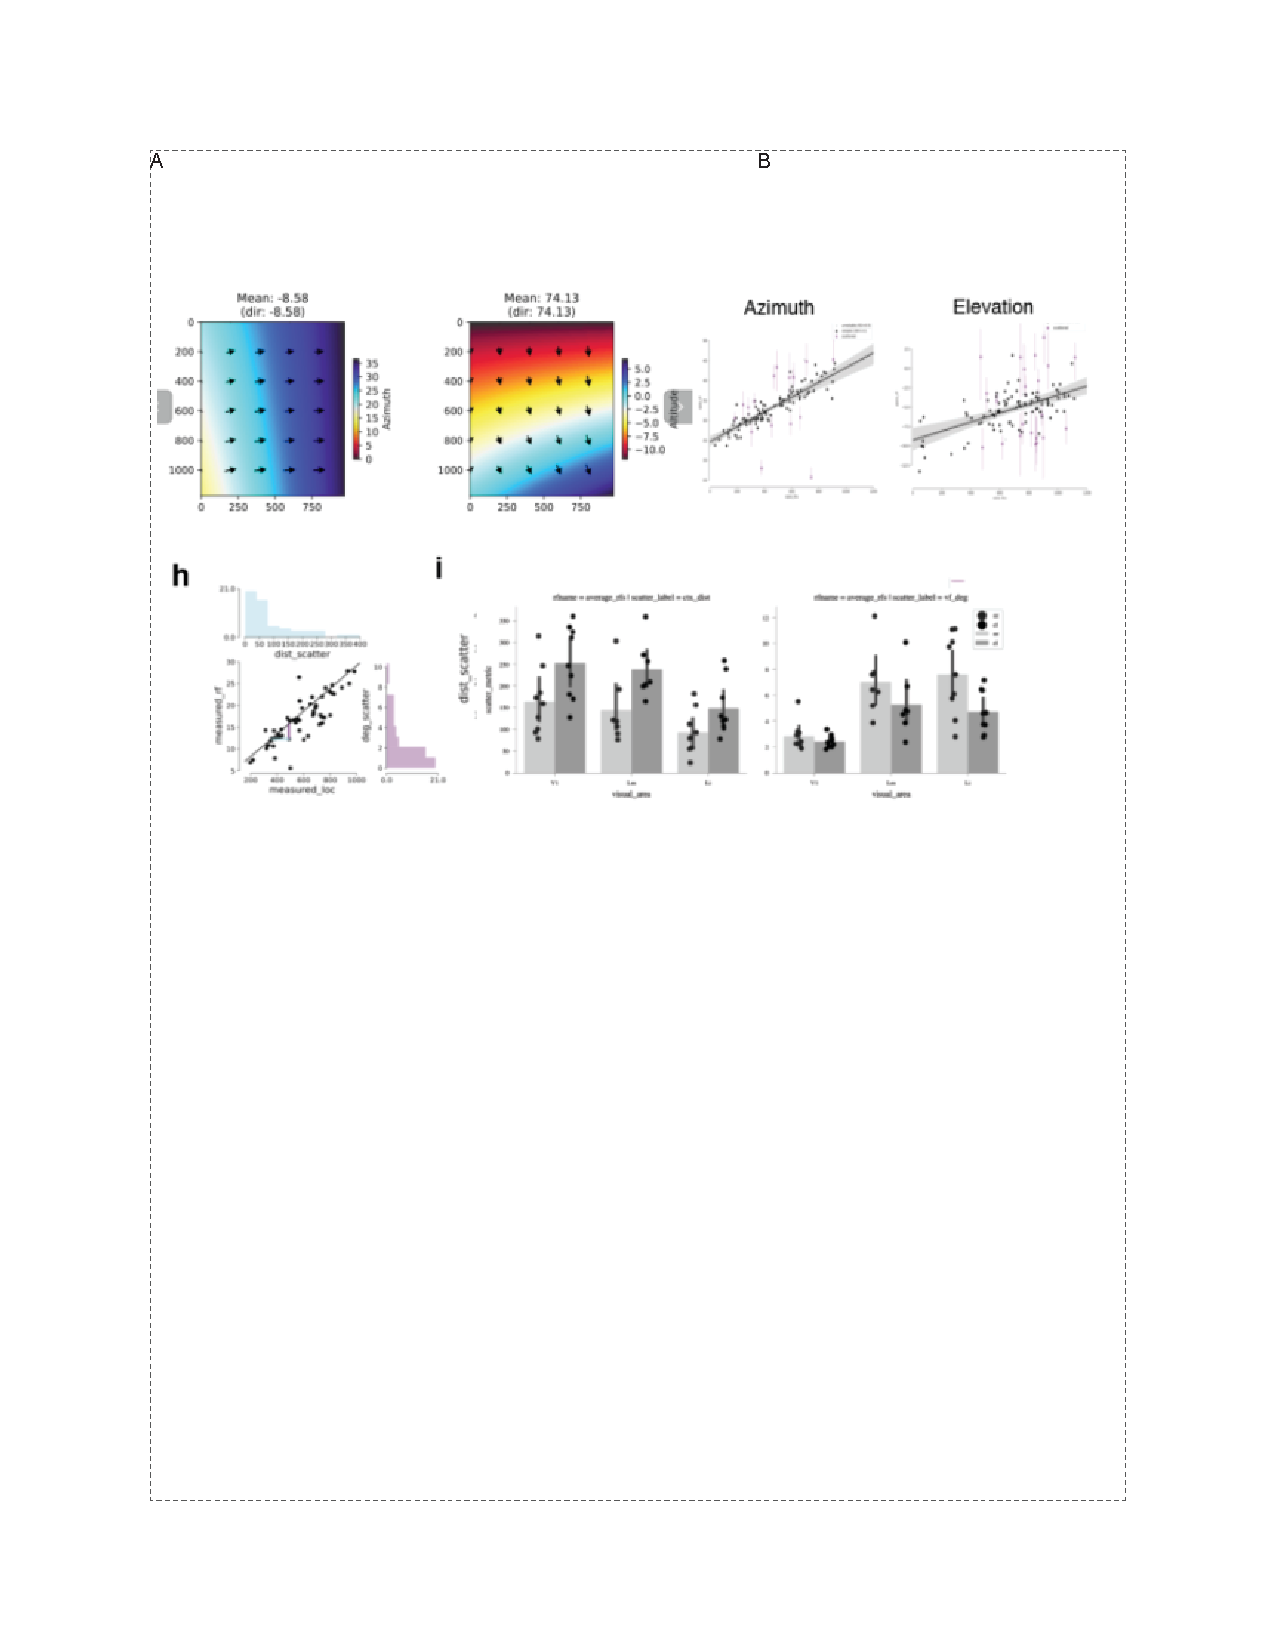
\includegraphics[width=\textwidth]{figures/chapter_3/retino_scatter/retino_scatter.pdf}
    \vspace{.1in}
    \caption[Fine-scale retinotopic organization]{Fine-scale retinotopic organization of lateral extrastriate cortex. \textbf{A.} REFREF.
    \label{fig:retino_scatter}}
\end{figure}

Overall, average scatter in cortical space decreased from V1 to LM to LI (V1: ~$239.09+/-REFREFum$, Lm: ~$163.48+/-REFREFum$, Li: ~$127.17+/-REFREFum$), corresponding to increasing average retinotopic displacements (V1: ~$2.90+/-REFREF$ degrees, LM: ~$5.30+/-REFREF$ degrees, LI: ~$6.45+/-REFREF$ degrees of visual angles). This relative patterns is consistent with the increasingly smaller sizes of areas V1 to LM to LI (that is, larger area, more room for error). 

Interestingly, the amount of scatter in the predicted receptive field locations corresponded to roughly half or less than the average receptive field size of each visual area (REFREF, V1: ~$9.49+/-REFREF$, Lm: ~$10.61+/-REFREF$, LI: ~$13.25+/-REFREF$ degrees of visual angle). However, at the level of individual cells, we observed no correlation between receptive field size and retinotopic scatter (Supp Figure REFREF), stats, Pearson’s correlation, V1: REFREF, p=REFREF, Lm: REFREF, p=REFREF, Li: REFREF, p=REFREF).

% Asymmetric scatter
The observed retinotopic scatter was asymmetric between vertical and horizontal dimensions, as well:  deviation from predicated cortical locations was ~2 fold larger along elevation than azimuth (V1: REFREF in azimuth, REFREF in elevation; Lm: REFREF in azimuth, REFREF in elevation; Li: REFREF in azimuth, REFREF in elevation), consistent with the observed axis asymmetry in cortical magnification for all areas tested based on smoothed neuropil estimates. 

% Scatter of ~150um in azimuth and ~300um in elevation corresponded to average retinotopic displacements of roughly ~3deg along both azimuth and elevation visual field positions.

For example, average retinotopic displacements were similar along azimuth and elevation for V1, ~3 degrees of visual angle, but the corresponding scatter at the level of neighboring cells was greater for elevation (~250um) than azimuth (~150um REFREF). 

-what drives the error?
-cellular processes that don't have anything to do with what brain encodes, would expect error to be lower, in terms of cortical distance -- 1um horizontal, 2um vertical
-but error is constant with deg. of visual field, 
-error is not constant per unit cortex, it is constant per unit visual field
-org. of cells driven by retinotopic inputs -- if purely driven b

-better resolution in elevation? -- horizontally oblong

-same deg. of error in visual space
-error in positioning is the same-- similar error


% Maybe this is for better visual field coverage?
Given these observed biases in receptive field angle or anisotropy, cortical magnification, and retinotopic scatter, we wondered whether these irregularities might allow, for example, enhanced visual coverage. For all simultaneously recorded cells in a given imaging site, we compared how the distribution of receptive fields across the visual field changed if all irregularities were corrected. 

\begin{figure}[t!]
    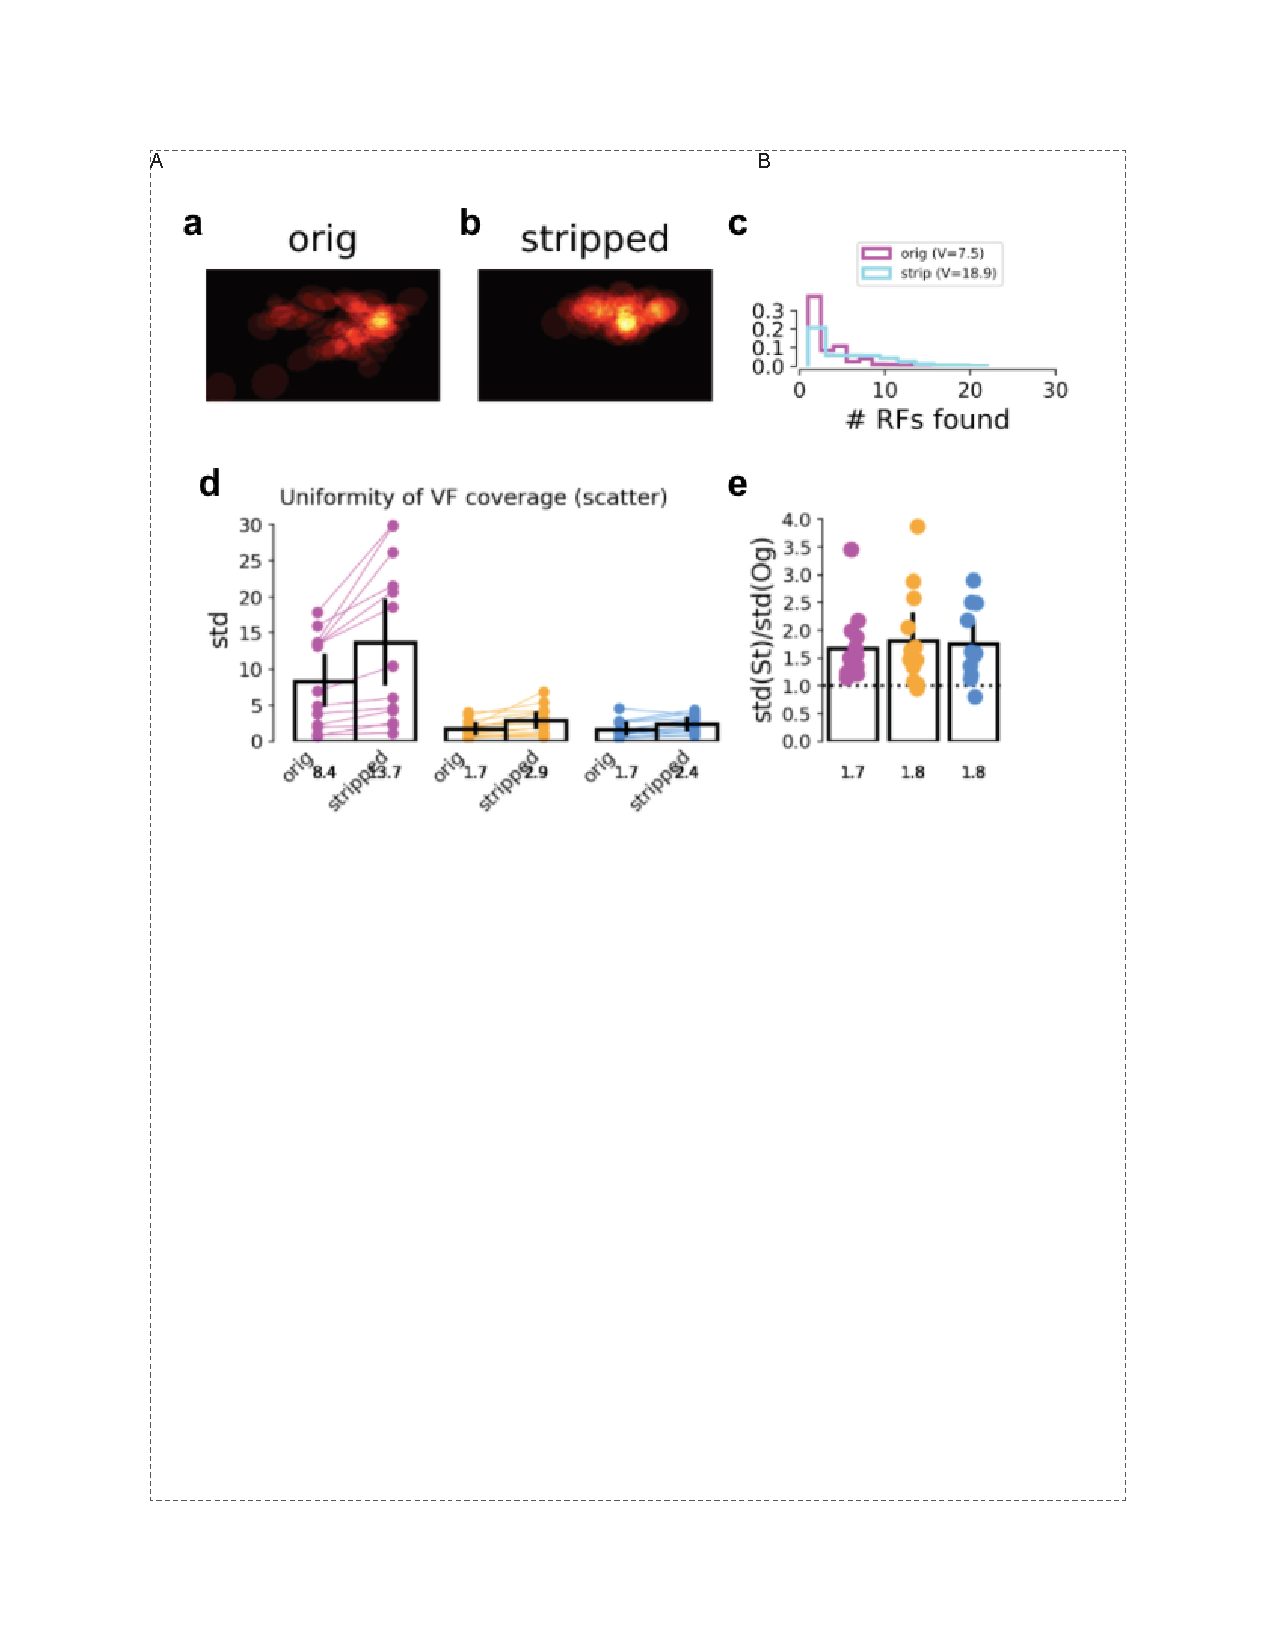
\includegraphics[width=\textwidth]{figures/chapter_3/vf_coverage/vf_coverage.pdf}
    \vspace{.1in}
    \caption[Compensatory visual field coverage]{Gains in visual field coverage due to scatter. \textbf{A.} REFREF.
    \label{fig:vf_coverage}}
\end{figure}

Specifically, to nullify retinotopic scatter, we assigned the predicted retinotopic position to each cell, and to nullify receptive field irregularities, we assigned size along each axis to be equal to the average of the two axes such that simulated receptive fields were perfectly isotropic (Figure\ref{fig:vf_coverage}). We calculated the variance of the distributions of RF counts across the visual field as a measure of how uniformly the receptive fields covered the visual field:  higher variance indicates RFs are clustered in select locations, while lower variance indicates RFs are evenly spread out (Figure\ref{fig:vf_coverage}). 

Overall, simulated RF distributions resulted in a less uniform visual field coverage than measured RF distributions (paired test REFREF, Figure\ref{fig:vf_coverage}). The fold-change in variance was greater than 1 (no difference) for all imaging sites (REFREF). %NO difference between areas?



% ---------------------------------------------------------------
% Gratings
% ---------------------------------------------------------------
\section{Orientation and direction tuning}
Since we did not observe retinotopic organization at the REFREF um scale, we asked whether neurons might be organized by tuning to other visual features. In highly visual animals, like primates and cats, orientation tuning exhibits a spatial organization in which columns of cortex show repeating "pinwheel" structures of preferred orientations\cite{REFREF}. In contrast, studies of rodent visual cortex have shown a disorganized, "salt-and-pepper" organization\cite{Ohki2005, REFREF}, even in more visual rodents like the squirrel\cite{VanHooser2005FunctionalRodent, REFREF}. The lack of clear global structure in one but the presence of clear orientation selectivity in both rodents and primates suggests that they represent alternative paths to achieving the same functionality.

To expand on known characteristics in rodent V1 to extrastriate areas in the rat, we measured calcium responses to drifting gratings of a range of directions, spatial frequencies, speeds, and sizes (Figure\ref{fig:gratings_examples}). 

\begin{figure}[t!]
    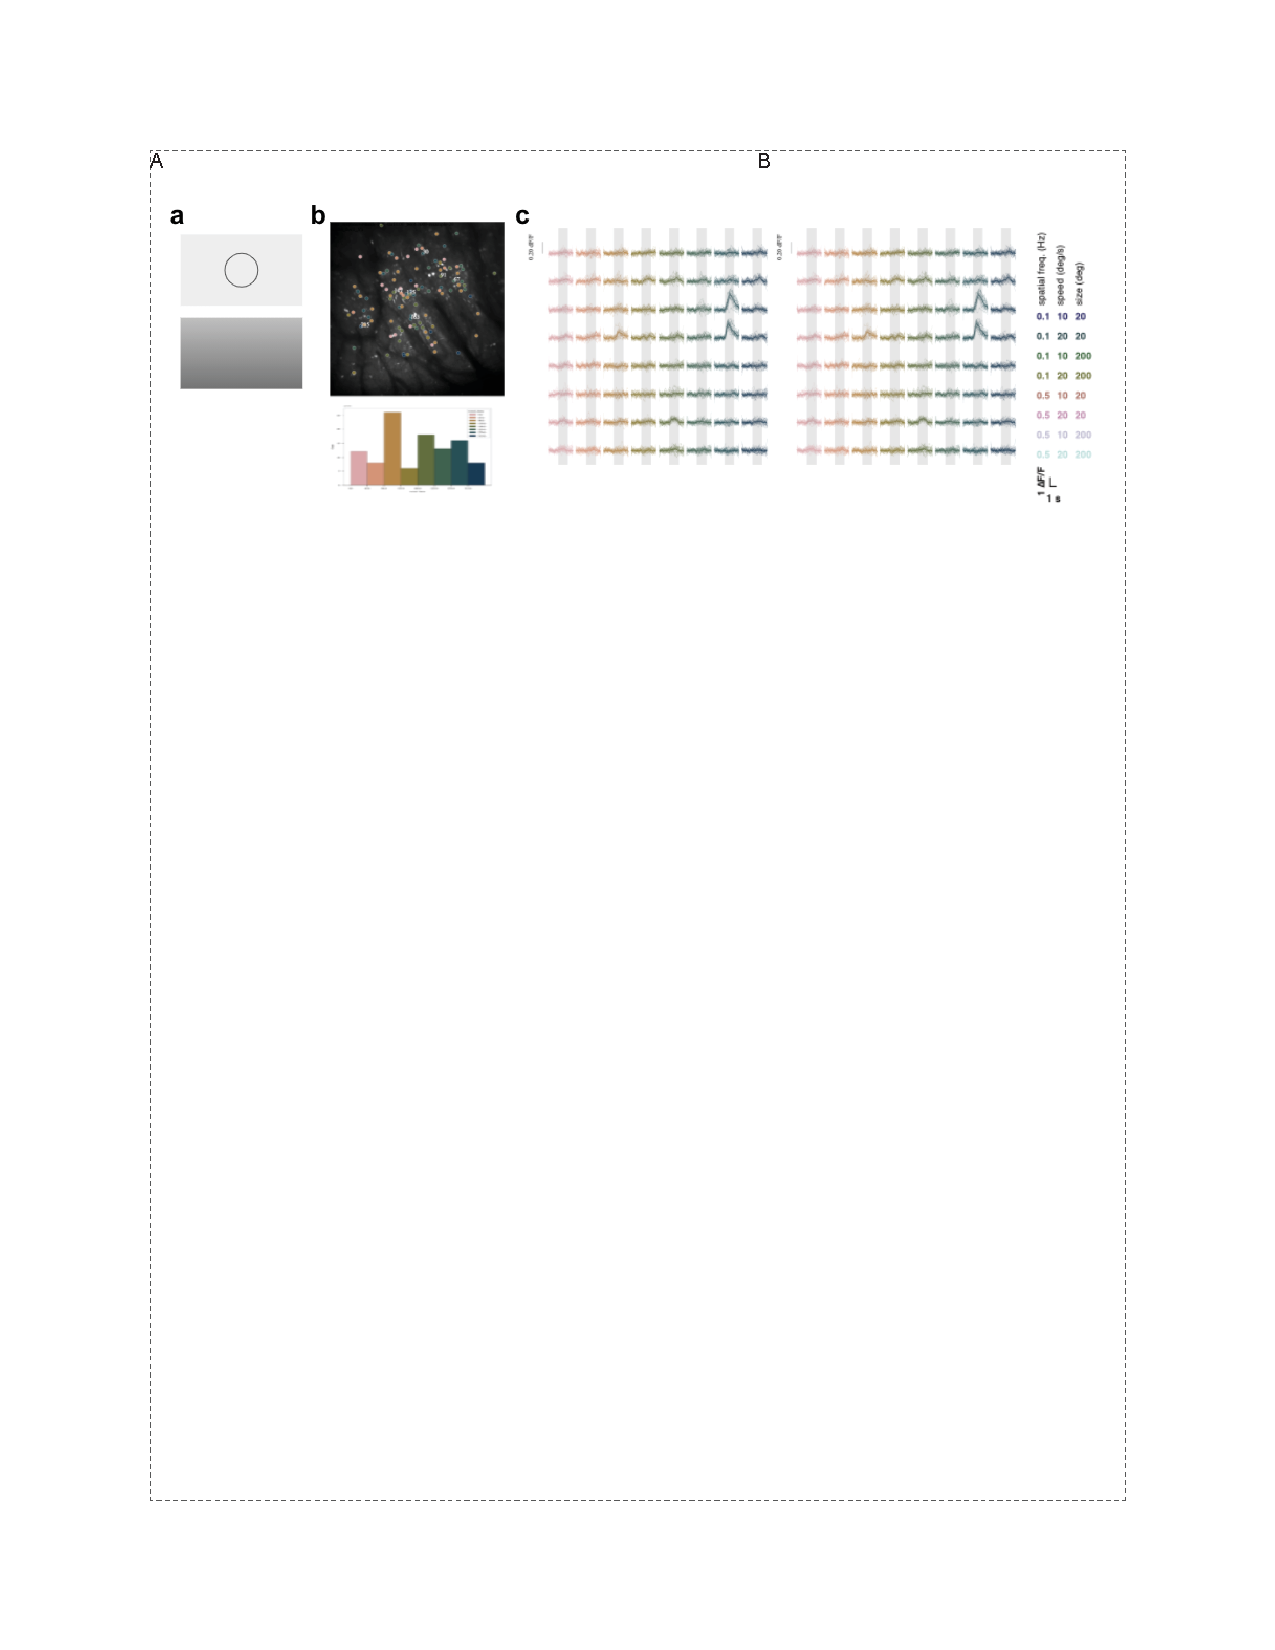
\includegraphics[width=\textwidth]{figures/chapter_3/gratings_example/gratings_examples.pdf}
    \vspace{.1in}
    \caption[Examples of feature tuning]{Examples of feature tuning. \textbf{A.} REFREF.
    \label{fig:gratings_examples}}
\end{figure}

Visually responsive cells were classified as responsive to a given direction of motion (direction-selective, DS), or to opposing directions of motion along a given axis (axis-selective, AS), or neither direction- or axis-selective (see Methods). Overall, we found that the fraction of cells tuned to axis or direction was significantly lower in area LI compared to V1 and LM REFREF (Figure\ref{fig:osi_dsi}). This apparent decrease for tuning to gratings was largely driven by a decrease in axis-selectivity, but not direction-selectivity (V1: REFREF+/-REFREF, n=REFRE; LM: REFREF+/-REFREF, n=REFREF; LI: REFREF+/-REFREF, n=REFREF). %slight increase in direction selectivity?

\begin{figure}[t!]
    \includegraphics[width=\textwidth]{figures/chapter_3/osi_dsi/osi_dsi.pdf}
    \vspace{.1in}
    \caption[Summary of feature tuning across lateral cortex]{Feature tuning in lateral cortex. \textbf{A.} REFREF.
    \label{fig:osi_dsi}}
\end{figure}

Across all imaging sites, we found a slight bias toward vertically-moving or horizontally-oriented gratings (Figure\ref{fig:osi_dsi}). REFREF compare with othres? Girman looks similar, but mouse like vertical stuff? check marques et al.


% Orientating tuning similarity v distance?
Consistent with previous studies in rats and other rodents, we found a rough salt-and-pepper organization in V1 FOVs, as well as LM and LI FOVs (REFREF). 
If visual areas exhibit a purely salt-and-pepper organization, tuning similarity and cortical distance should be statistically independent. To quantify the similarity in tuning between cells, we created an average tuning profile for each cell, defined as the trial-averaged response to each condition, and measured similarity as the correlation coefficient between tuning profiles (Methods). The cortical distance between cells was defined as the distance between each cell’s center of mass in the image plane. 

\begin{figure}[t!]
    \includegraphics[width=\textwidth]{figures/chapter_3/ori_distance/ori_distance.pdf}
    \vspace{.1in}
    \caption[Organization of tuning similarity]{Signal correlations and spatial organization. \textbf{A.} CC as a function of cortical distance. \textbf{B.} CC as a function of receptive field overlap. \textbf{C.} Noise corrs??
    \label{fig:ori_distance}}
\end{figure}

Rather than a purely random organization of orientation preferences, we found a decrease in tuning similarity as a function of distance (Figure\ref{fig:ori_distance}). 

% Signal correlations vs. percent-overlap?.
To determine the extent to which similarity in tuning might be explained by receptive field organization, we looked at signal correlations as a function of receptive field overlap. 

% Axis/Direction tuning vs RF orientation?
Given the observed anisotropies in receptive field shape, we asked whether a cell's direction or axis preference was related to the orientation or angle of its receptive field. That is, a cell highly tuned to vertical (upward or downward) motion might have a receptive field elongated along the vertical dimension, parallel to the preferred direction of motion. On the other hand, the receptive field might be elongated along the axis perpendicular to direction of motion, \textit{i.e.}, horizontally elongated, reflecting the cell's preferred tuning to horizontal edges, 

\begin{figure}[t!]
    \includegraphics[width=\textwidth]{figures/chapter_3/ori_rfs/ori_rfs.pdf}
    \vspace{.1in}
    \caption[Receptive field shape and edge tuning]{Feature tuning in lateral cortex. \textbf{A.} REFREF.
    \label{fig:ori_rfs}}
\end{figure}

Overall, we found that receptive field orientations roughly matched axis preferences of neurons in V1 (Figure\ref{fig:ori_rfs}). 

